\documentclass[a4paper,11pt]{article}
\usepackage[utf8]{inputenc}
\usepackage[left=2cm,text={17cm,24cm},top=3cm]{geometry}
\usepackage{times}
\usepackage[czech]{babel}
\usepackage[ruled, czech, noline, longend, linesnumbered]{algorithm2e}
\usepackage{graphicx}
\begin{document}
\graphicspath{ {./etiopan.eps}{./oniisan.eps}{./oniisan2.eps} }


\begin{center}
\thispagestyle{empty}
\setcounter{page}{0}
\Huge
\textsc{Vysoké učení technické v~Brně \\ \huge Fakulta informačních technologií}\\
\vspace{\stretch{0.382}}
\huge Typografie a publikování -- 3. projekt \\
\Huge{Tabulky a obrázky}
\vspace{\stretch{0.618}}
\end{center}
{\large \today \hfill
Štěpán Czajkowski}
\newpage

\section{Úvodní strana}
Název práce umístěte do zlatého řezu a nezapomeňte uvést „dnešní“ datum a vaše jméno a příjmení.

\section{Tabulky}
Pro sázení tabulek můžete použít buď prostředí \texttt{tabbing} nebo prostředí \texttt{tabular}.

\subsection{Prostředí \texttt{tabbing}}
Při použítí \texttt{tabbing} vypadá tabulka následovně:

\begin{tabbing}
\verb|\pushtabs|\qquad \= \qquad \quad \= \kill
\textbf{Ovoce} \>\textbf{Cena} \>\textbf{Množství} \\
Jablka         \>25,90         \>3 kg              \\
Hrušky         \>27,40         \>2,5 kg            \\
Vodní melouny  \>35,--         \>1 kus

\end{tabbing}
Toto se dá také použít pro sázení algoritmů, ovšem vhodnější je použít prostředí \texttt{algorithm} nebo \\\texttt{algorithm2e} (viz sekce 3). 

\subsection{prosředí \texttt{tabular}}
Další možností, jak vytvořit tabulku, je použítí prostředí \texttt{tabular}. Tabulky pak budou vypadat takto\footnote{Kdyby byl problém s~\texttt{cline}, zkuste se podívat třeba sem: http://www.abclinuxu.cz/tex/poradna/show/325037.}:

\begin{table}[ht]
\begin{center}
\catcode`\-=12
\begin{tabular}{|l|ll|}
\hline
\multicolumn{1}{|c|}{} & \multicolumn{2}{c|}{\textbf{Cena}}                            \\ \cline{2-3} 
\textbf{Měna}          & \multicolumn{1}{l|}{\textbf{nákup}}     & \textbf{prodej}     \\ \hline
EUR                    & \multicolumn{1}{l|}{24,775}             & 25,943              \\ 
GBP                    & \multicolumn{1}{l|}{29,394}             & 30,492              \\ 
USD                    & \multicolumn{1}{l|}{22,423}             & 23,661              \\ \hline
\end{tabular}
\caption{Tabulka kurzů k~dnešnímu dni}
\label{table:1}
\end{center}
\end{table}

\begin{table}[h]
    \centering
    \begin{tabular}{|l|l|}
    \hline
    $A$ & $\neg A$ \\ \hline
    P & N    \\ \hline
    O~& O~\\ \hline
    X & X    \\ \hline
    N & P    \\ \hline
    \end{tabular}
    \caption{Protože Kleeneho trojhodnotová logika už je „zastaralá“, uvádíme si zde příklad čtyřhodnotové logiky}
    \label{table:2}
\end{table}

\newpage
\section{Algoritmy}
Pokud budete chtít vysázet algoritmus, můžete použít prostředí \texttt{algorithm}\footnote{Pro nápovědu, jak zacházet s~prostředím \texttt{algorithm}, můžete zkusit tuhle stránku:\\http://ftp.cstug.cz/pub/tex/CTAN/macros/latex/contrib/algorithms/algorithms.pdf.} nebo \texttt{algorithm2e}\footnote{Pro \texttt{algorithm2e} zase tuhle: http://ftp.cstug.cz/pub/tex/CTAN/macros/latex/contrib/algorithm2e/doc/algorithm2e.pdf.}. Příklad použítí prostředí \texttt{algorithm2e} viz Algoritmus \ref{alg1}.
%\SetAlCapSkip{1em}
\SetKwInput{KwInput}{Input}
\SetKwInput{KwOutput}{Output}

\begin{algorithm}[ht]
    \SetAlgoLined
    \KwInput{$(X_{t-1},u_t,z_t)$}
    \KwOutput{$X_t$}

    $\overline{X_t} = X_t = 0$\\
    {\For{$k\gets0$ \KwTo $M$}{
     $x^{[k]}_t = sample\_motion\_mode(u_t,x^{[k]}_{t-1})$\\
     $w_t^{[k]} = measurement\_model(z_t,x^{[k]}_t,m_{t-1}^{[k]} )$\\
     $m_t^{[k]} = updated\_occupancy\_grid(z_t,x_t^{k},m_{t-1}^{[k]})$\\
     $\overline{X_t} = \overline{X_t} + \langle x_x^{[m]}, w_t^{[m]} \rangle$
    }}
    {\For{$k\gets0$ \KwTo $M$}{
        draw $i$ with probability $\approx w_t^{[i]}$ \\
        add $\langle x_x^{[k]}, w_t^{[k]} \rangle$ to $X_t$
    }}
    \caption{\textsc{FastSlam}}\label{alg1}
    \KwRet{$X_t$}
\end{algorithm}

\section{Obrázky}
Do našich článků můžete samozřejmě vkládat obrázky. Pokud je obrázkem fotografie, můžete klidně použít bitmapový soubor. Pokud by to ale mělo být nějáké schéma nebo něco podobného, je dobrým zvykem takovýto obrázek vytvořit vektorově.
\begin{figure}[ht]
    \centering
    \scalebox{0.45}{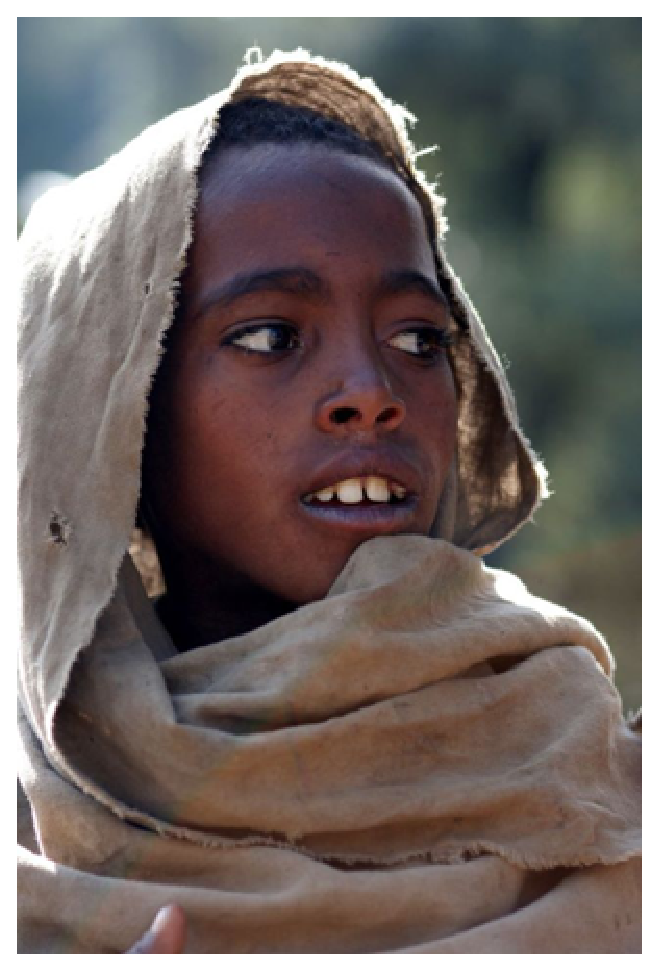
\includegraphics{etiopan.eps}}
    \reflectbox{\scalebox{0.45}{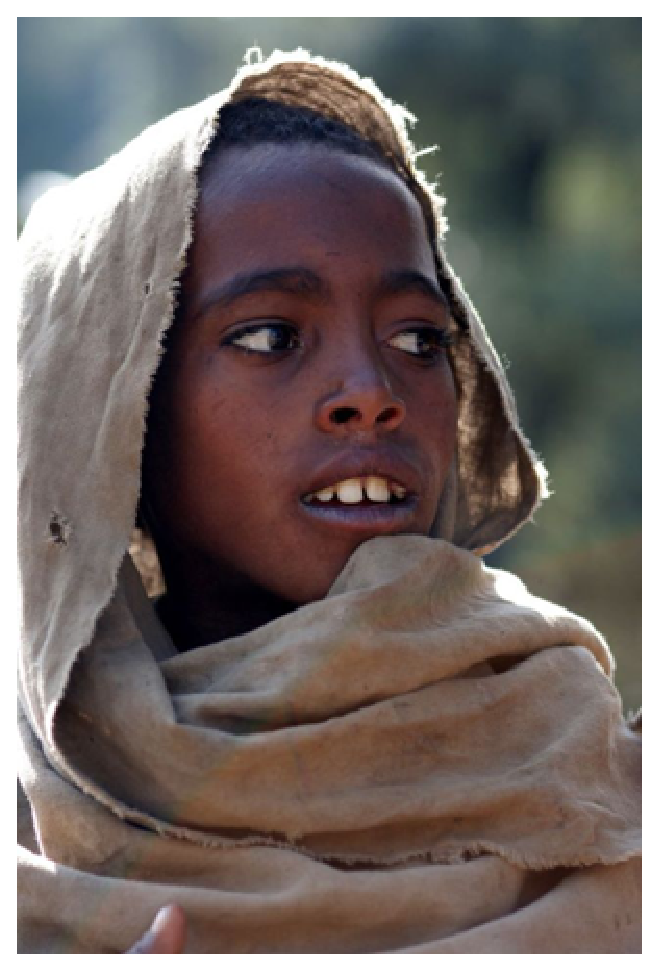
\includegraphics{etiopan.eps}}}
    \caption{Malý Etiopánek a jeho bratříček}
    \label{fig:0}
\end{figure}

\newpage
Rozdíl mezi vektorovým $\dots$
\begin{figure}[ht]
    \centering
    
\includegraphics[height=2cm,width=8cm]{oniisan.eps}
    \caption{Vektorový obrázek}
    \label{fig:2}
\end{figure}

$\dots$ a bitmapovým obrázkem
\begin{figure}[ht]
    \centering
    
\includegraphics[height=2cm,width=8cm]{oniisan2.eps}
    \caption{Bitmapový obrázek}
    \label{fig:3}
\end{figure}

se projeví například zvětšením.\\
Odkazy (nejen ty) na obrázky \ref{fig:0}, \ref{fig:2}, \ref{fig:3}, na tabulky \ref{table:1} a \ref{table:2} a také na algoritmus 1 jsou udělány pomocí křížkových odkazů. Pak je ovšem potřeba zdrojový soubor přeložit dvakrát.\\
Vektorové obrázky lze vytvořit i přímo v~\LaTeX u, například pomocí prostředí \texttt{picture}.
\end{document}
\newpage

\begin{figure}
    \centering
    \includegraphics{}
    \caption{Vektorový obrázek moderního bydlení vhodného pro 21. století. (Buďto vytvořte stejný obrázek, anebo nakreslete pomocí \texttt{picture} váš vlastní domov.)}
    \label{fig:4}
\end{figure}